\documentclass[12px]{article}
\usepackage{hyperref}
\usepackage{graphicx}
\usepackage{fancyhdr}
\usepackage{geometry}
	\geometry{height=24 cm}
	\geometry{left=2.5 cm}
	\geometry{right=2.5 cm}
	\geometry{top=2 cm}
	\geometry{headheight=1 cm}

\setcounter{secnumdepth}{1}

\title{Relazione di laboratorio}
\author{Carlo Rosso \\ n. matricola: 2034293}


\begin{document}
\begin{titlepage}
	\maketitle
	\thispagestyle{empty}
\end{titlepage}

Dal momento che non sono riuscito a essere presente alla lezione di laboratorio tenutasi il 31 maggio, segue una relazione sul laboratorio che riguarda le politiche di gestione della memoria virtuale.\\

In breve, effettuo un confronto tra le politiche di gestione della memoria virtuale, portando esempi di politiche più efficaci in alcune circostanze e meno in altre. La mia analisi riguarda solamente l'efficienza degli algoritmi utilizzato.\\
In questo esempio, osserviamo alcune statistiche relative a ciascun algoritmo mentre è simulata l'esecuzione di 7 processi con tempo di arrivo e durata scelti (scelti nel senso che deciderò io il tempo di arrivo e la durata di ciascuno, influenzando l'analisi, per mettere in luce le caratteristiche principali degli algoritmi).

\subsubsection{Settaggio}
Per quanto riguarda la configurazione iniziale è stata impostata come segue dalle figure:
\begin{figure}[h]
	\centering
	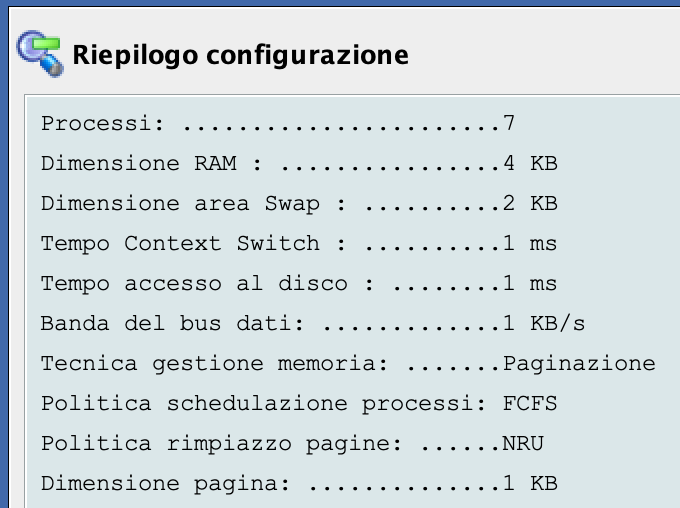
\includegraphics[scale=0.3]{img/impostazioni}
	\caption{Impostazioni generiche.}
\end{figure}

Di seguito sono riportati i tempi di arrivo e le durate di ciascun processo.
\begin{figure}[h]
	\centering
	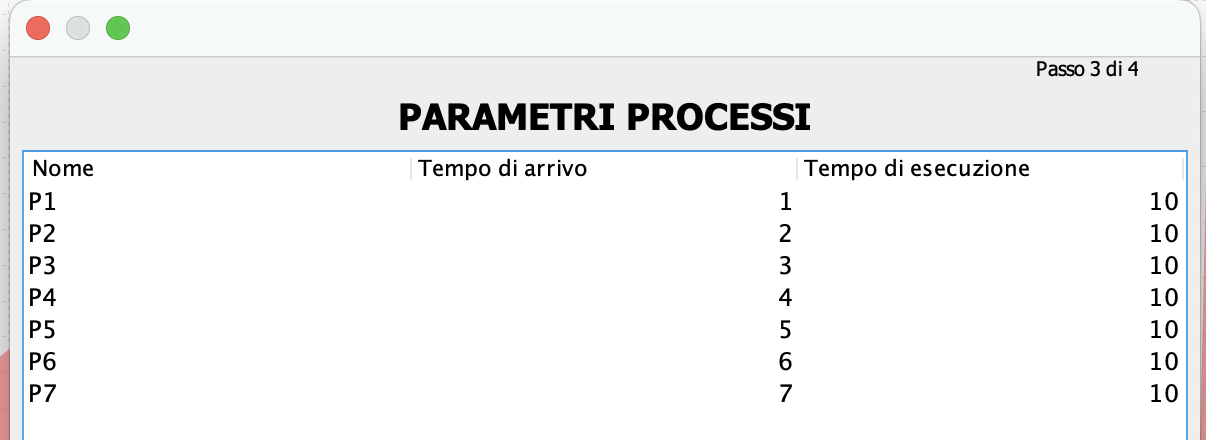
\includegraphics[scale=0.25]{img/durata}
	\caption{tempo di arrivo e durata di ciascun processo.}
\end{figure}

Ho deciso di utilizzare come esempio solo processi che durano 10 istanti perchè in questo modo i grafici completi sono più facilmente confrontabili.

Infine sono elencate le pagine richieste in ciascun momento da ogni processo.
% elenco della richiesta delle pagine
    \begin{figure}[!h]
        \centering
        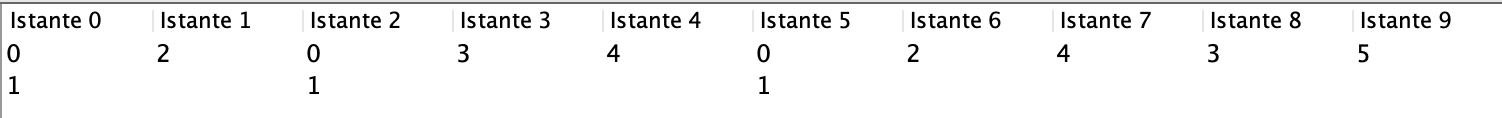
\includegraphics[scale=0.3]{img/1}
        \caption{Tempo di arrivo e durata del processo 1.}
    \end{figure}

    \begin{figure}[!h]
        \centering
        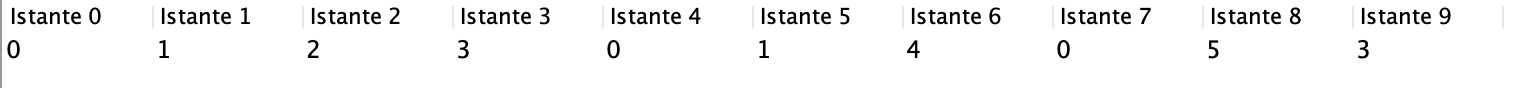
\includegraphics[scale=0.3]{img/2}
        \caption{Tempo di arrivo e durata del processo 2.}
    \end{figure}

    \begin{figure}[!h]
        \centering
        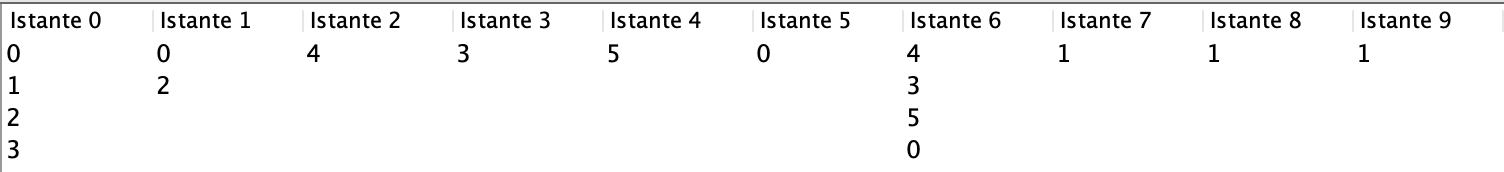
\includegraphics[scale=0.3]{img/3}
        \caption{Tempo di arrivo e durata del processo 3.}
    \end{figure}

    \begin{figure}[!h]
        \centering
        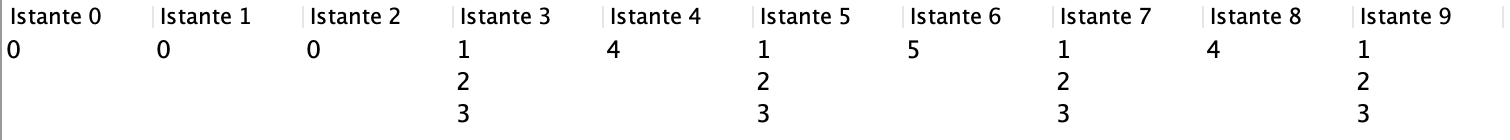
\includegraphics[scale=0.3]{img/4}
        \caption{Tempo di arrivo e durata del processo 4.}
    \end{figure}

    \begin{figure}[!h]
        \centering
        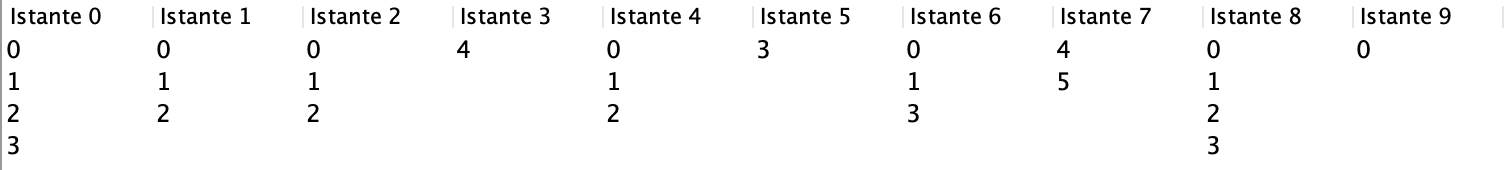
\includegraphics[scale=0.3]{img/5}
        \caption{Tempo di arrivo e durata del processo 5.}
    \end{figure}

    \begin{figure}[!h]
        \centering
        
\includegraphics[scale=0.3]{img/6}
        \caption{Tempo di arrivo e durata del processo 6.}
    \end{figure}

    \begin{figure}[!h]
        \centering
        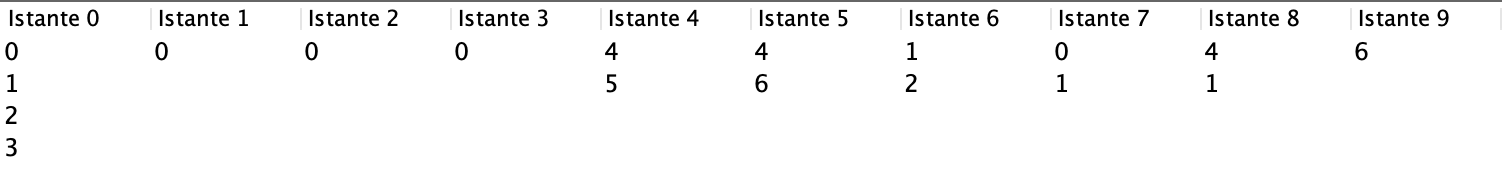
\includegraphics[scale=0.3]{img/7}
        \caption{Tempo di arrivo e durata del processo 7.}
    \end{figure}

\subsection{Raccolta Dati}
Ora non resta che far partire il programma, per leggere i dati ed interpretarli. Come anticipavo, mi limiterò a cambiare solamente la politica di rimpiazzo delle pagine, per evidenziare le differenze solamente tra le politiche di rimpiazzo delle pagine.

Di seguito sono riportati i grafici delle statistiche sui page fault riguardo alle politiche di ordinamento viste a lezione.

\begin{figure}[!h]
	\centering
	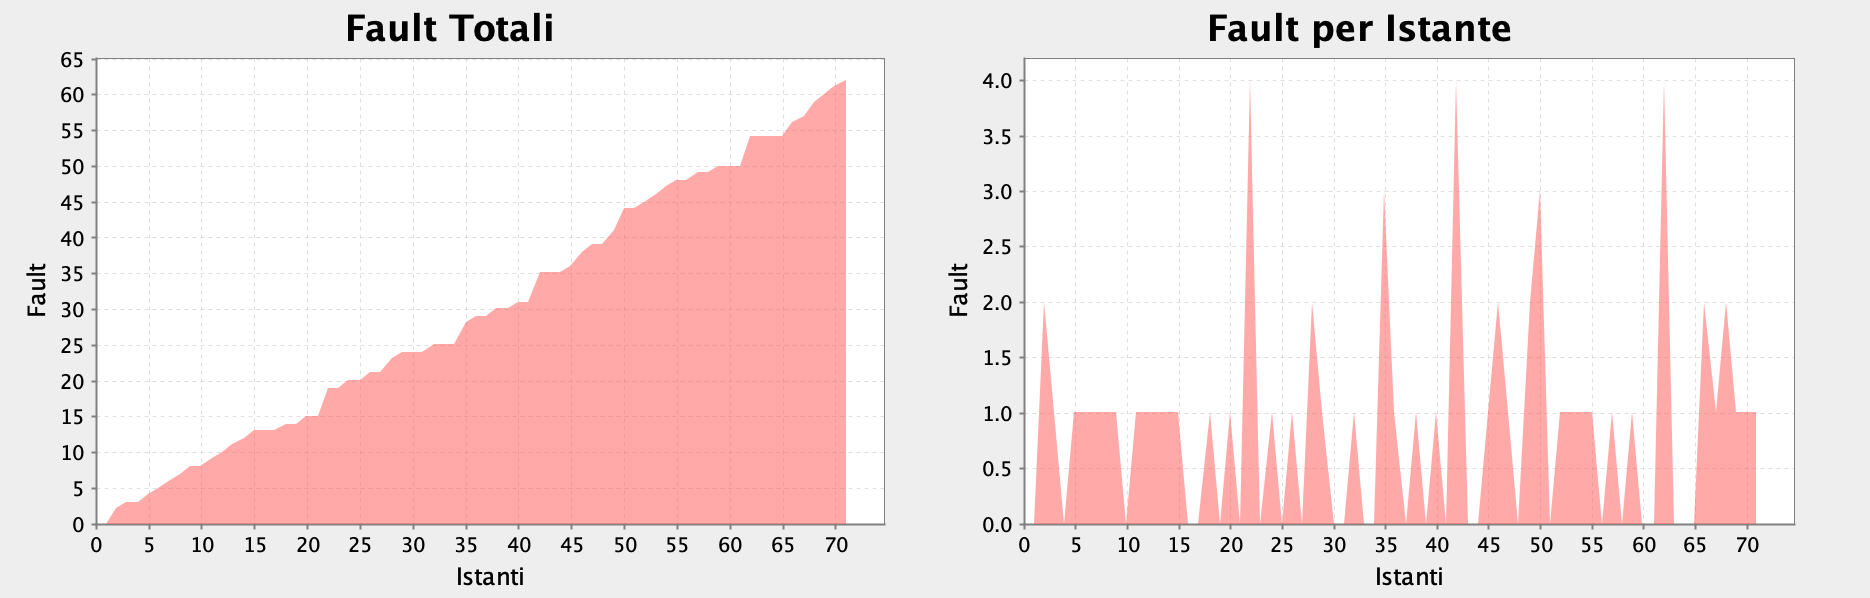
\includegraphics[scale=0.3]{img/nru}
	\caption{Not Recently Used}
    \label{fig:NRU}
\end{figure}

\begin{figure}[!h]
	\centering
	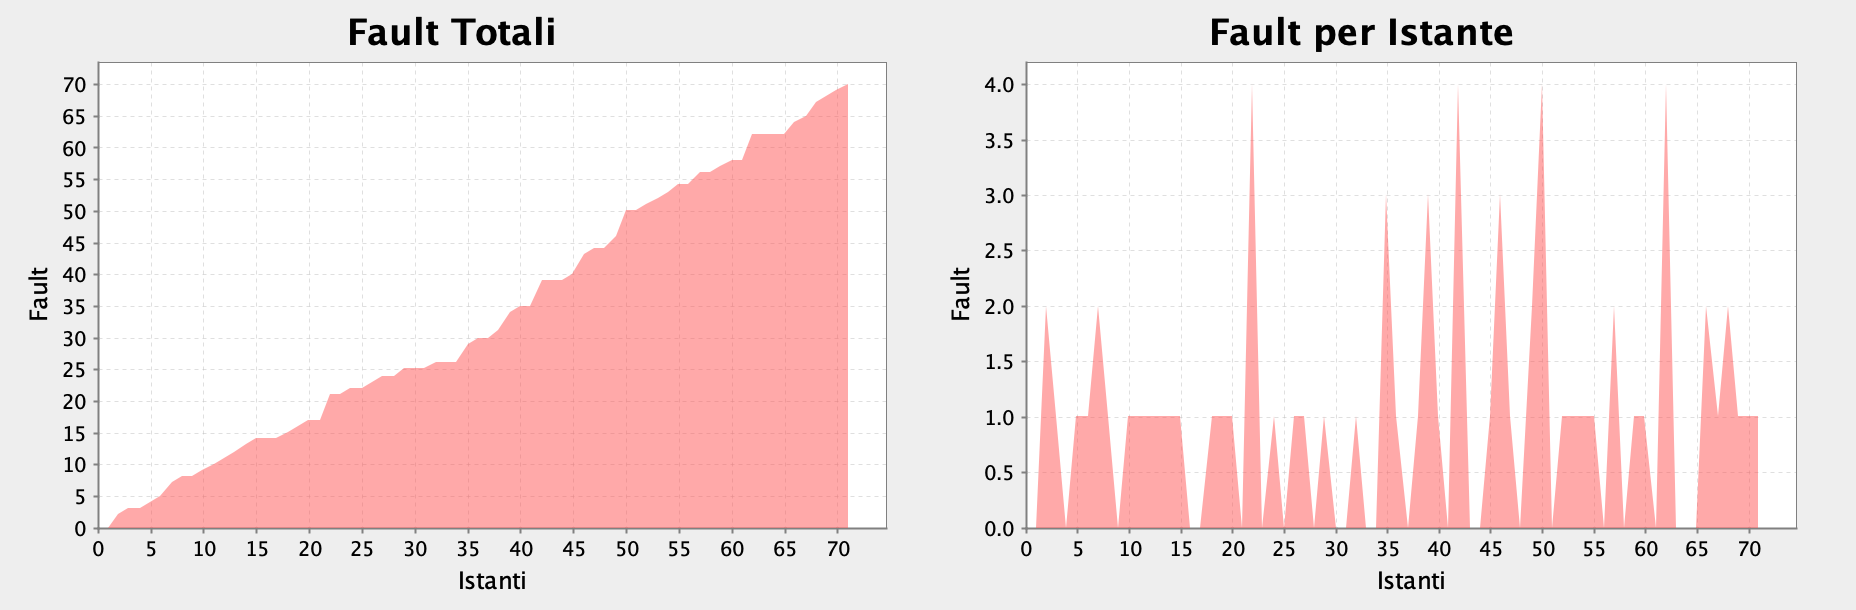
\includegraphics[scale=0.3]{img/fifo}
	\caption{First In First Out}
    \label{fig:FIFO}
\end{figure}

\begin{figure}[!h]
	\centering
	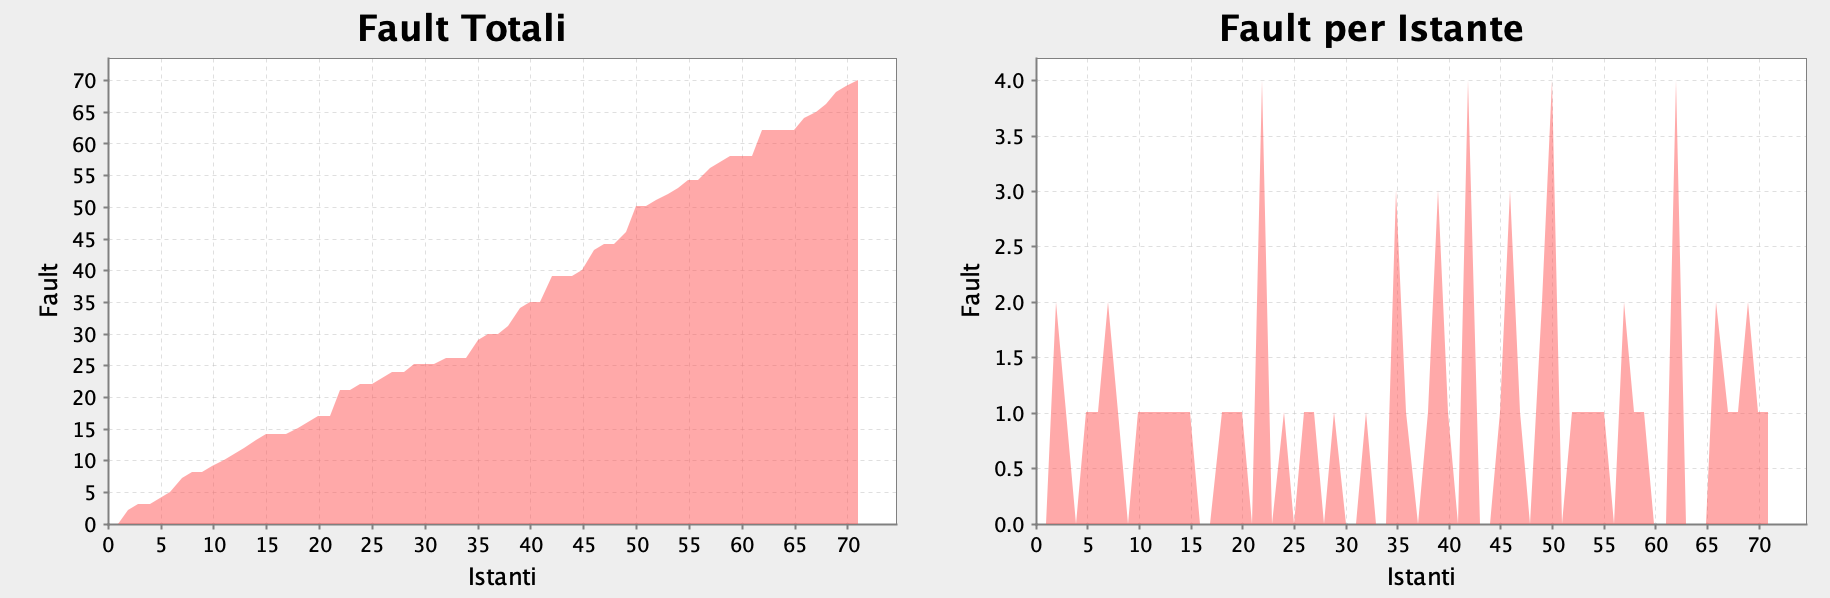
\includegraphics[scale=0.3]{img/sc}
	\caption{Second Chance}
    \label{fig:SC}
\end{figure}

\begin{figure}[!h]
	\centering
	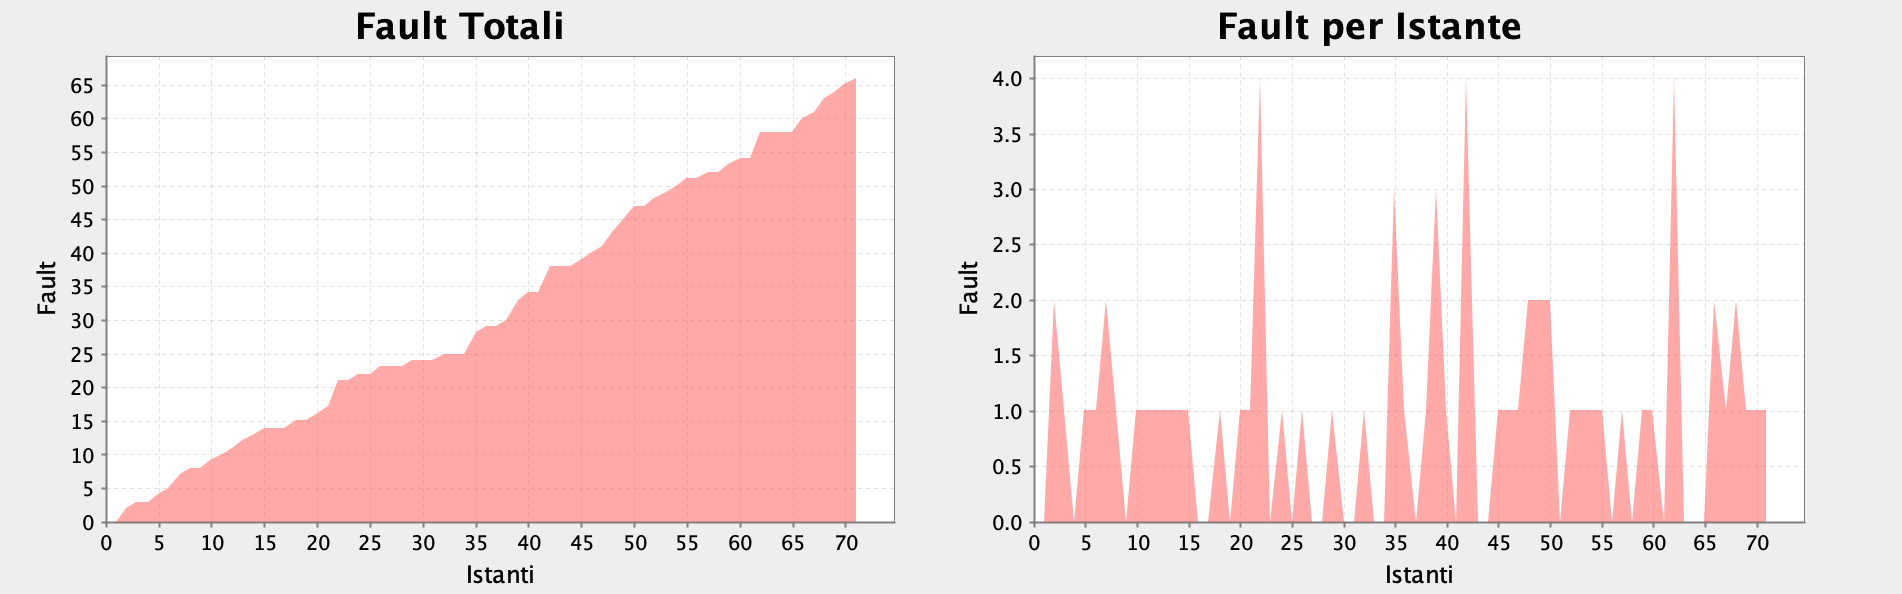
\includegraphics[scale=0.3]{img/c}
	\caption{Clock}
    \label{fig:C}
\end{figure}

\begin{figure}[!h]
	\centering
	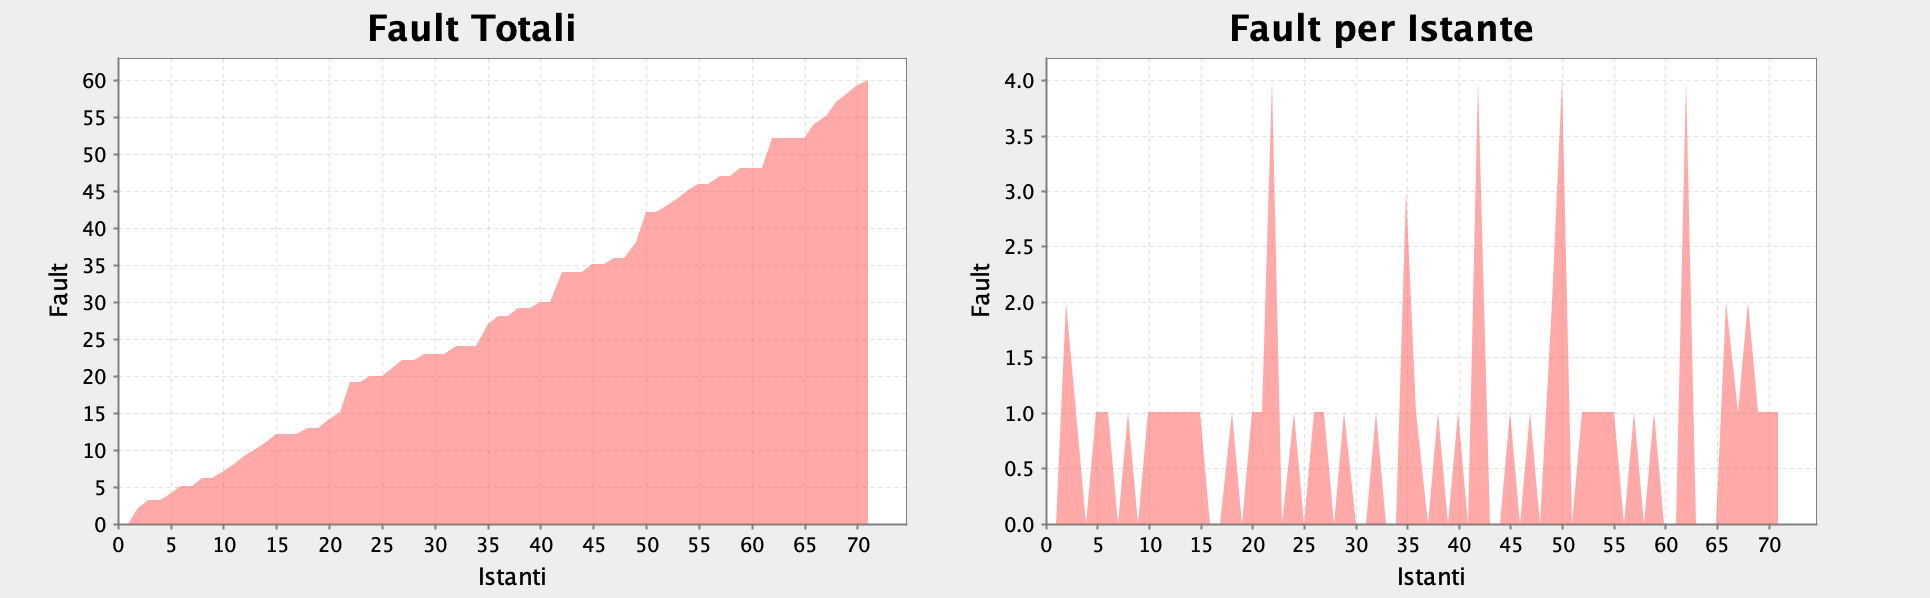
\includegraphics[scale=0.3]{img/lru}
	\caption{Least Recently Used}
    \label{fig:LRU}
\end{figure}

\begin{figure}[!h]
	\centering
	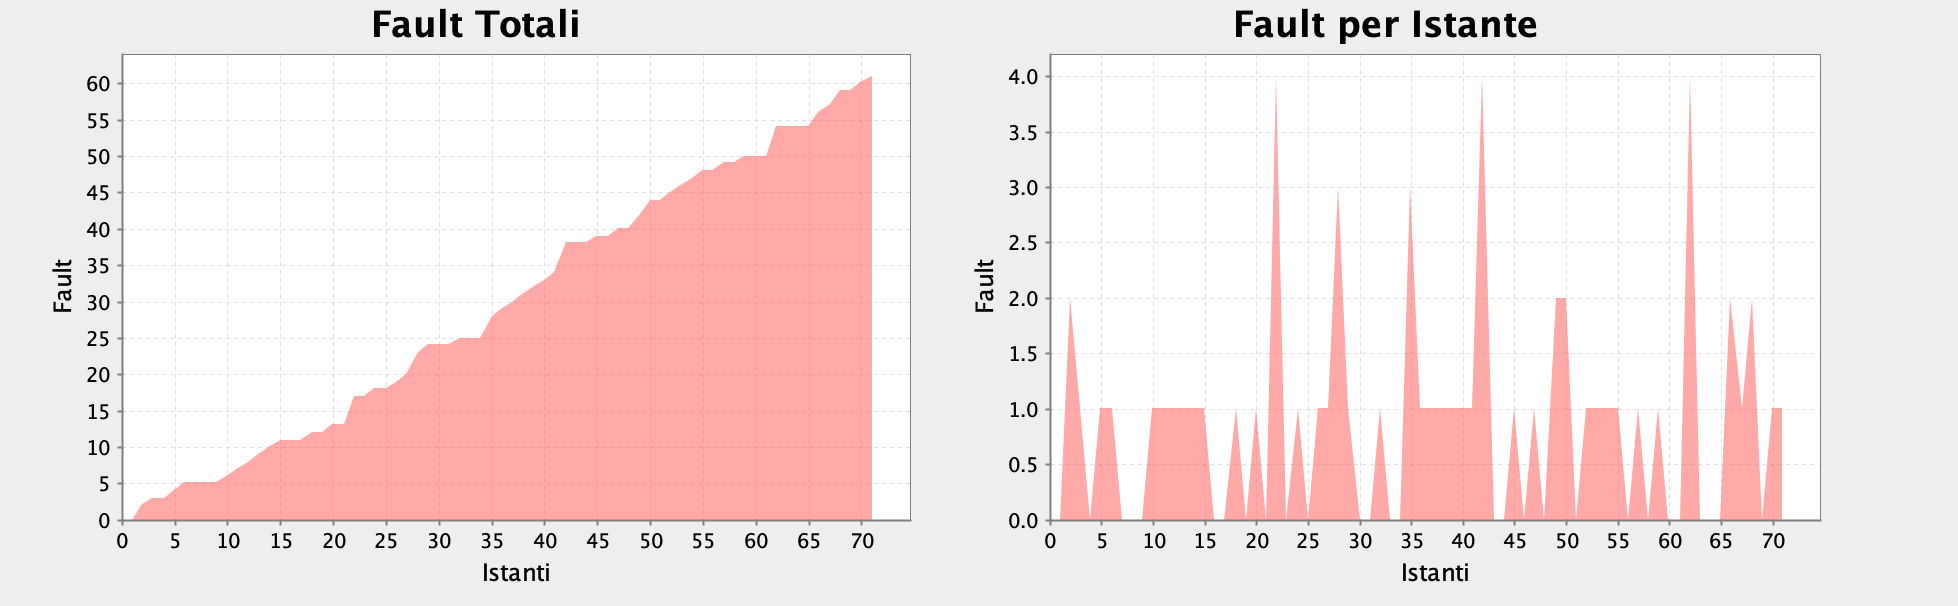
\includegraphics[scale=0.3]{img/nfu}
	\caption{Not Frequently Used}
    \label{fig:NFU}
\end{figure}

\begin{figure}[!h]
	\centering
	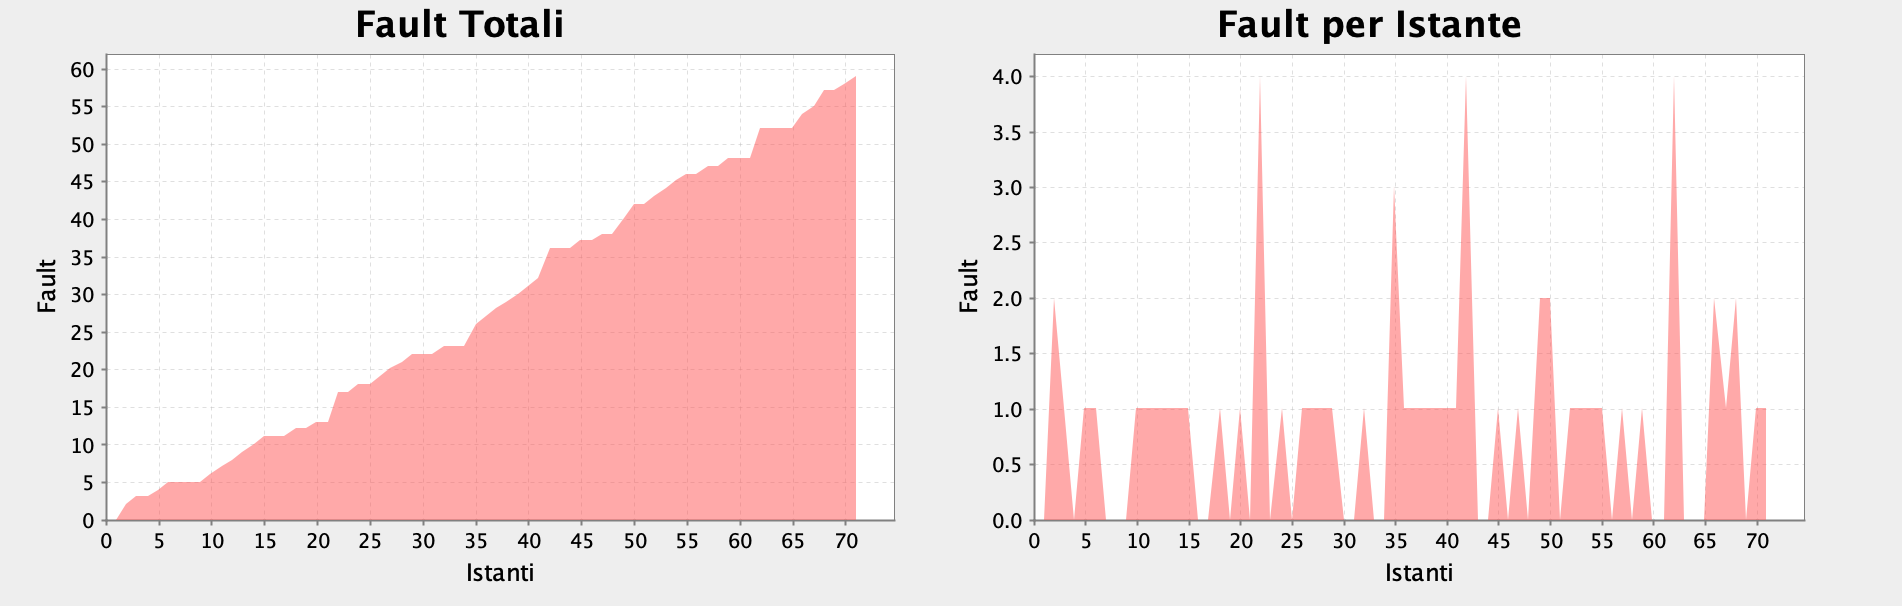
\includegraphics[scale=0.3]{img/a}
	\caption{Aging}
    \label{fig:A}
\end{figure}
\newpage
\section{Analisi dei dati}
A primo approccio, in un confronto generale, comprendiamo la politica che effettua meno page fault osservando la scala di misura dei fault nel grafico dei fault totali. In questo modo, risulta evidente che gli ultimi tre grafi, che raffigurano i page fault rispettivamente delle politiche Least Frequently u
Used, Not frequently Used e Aging, rappresentano le politiche migliori. In particolare il grafico \ref{fig:NFU} indica un numero di page fault totali appena superiori ai 60; mentre il grafico \ref{fig:LRU} rappresenta una politica che totalizza proprio 60 page fault. Infine, la politica aging, con le impostazioni riportare risulta completare i processi col minor numero di page fault tra le politiche di ordinamento analizzate (meno di 60).\\

Osservando le impostazioni di partenza, in particolare il numero di processi, la loro durata e l'ordine, notiamo che sono svolti in ordine dal primo all'ultimo ed ognuno ha una durata di 10 istanti. Queste impostazioni sono state scelte per permettere un confronto più preciso tra i vari istanti. Il resto dell'analisi consiste proprio in un confronto per quanto riguarda l'esecuzione dei singoli processi. 

\subsection{Istanti 1-10}
Nei primi 10 istanti viene eseguito completamente il primo processo. Il primo processo servirebbe per mostrare come funziona la politica Not Recently Used. Non è possibile illustrare bene il suo funzionamento in quanto non si riesce ad indicare quali blocchi siano usati in lettura e quali in scrittura. Si tratta di un'approssimazione dell'effettiva politica di scelta delle pagine in memoria principale.\\
Per quanto riguarda la politica Not Recently Used, notiamo che in totale avvengono 9 page fault in RAM (il grafico non rende bene l'idea, ma lo si può calcolare dai dati iniziali). L'utilizzo delle pagine è stato scelto per far spiccare questa politica, ma a discapito di quanto si potrebbe pensare non si tratta della politica migliore. Questo in realtà non è strano: la politica di ripiazzo delle pagine Not Recently Used è un'approssimazione più semplice della politica Least Recently Used, che risulta essere migliore della copia. Gli algoritmi che si comportano meglio in queste impostazioni sono proprio quelli che derivano dalla Least Recently Used: Aging (figura \ref{fig:A}) e Not Frequently Used (figura \ref{fig:NFU}). Mentre hanno il medesimo numero di page fault le politiche FIFO, Second Chance e Clock (figure: \ref{fig:FIFO}, \ref{fig:SC}, \ref{fig:C}). Mi aspettavo un risultato di questo tipo perchè effettivamente l'idea alla base di questi algoritmi è piuttosto diversa dal resto degli algoritmi: si basano sull'ordine di arrivo, piuttosto che sull'ultima volta in cui il processo è stato utilizzato.

\subsection{Istanti 11-20}
Nella seconda decina di istanti, viene eseguito il secondo processo. In questo caso avviene un pagefault per i primi 4 istanti, dopo i quali non ci sono pagefault per i successivi 2 istanti ed avviene il successivo page fault quando è richiesta la pagina 4. Questo avviene per tutti i processi. All'istante 7 avviene la richiesta in lettura o scrittura della pagina 0 che è stata riferita l'ultima volta all'istante 15, ma è entrata in ram per la prima volta all'istante 11. Per questo motivo si cominciano a dividere le politiche in base ai page fault solo in questo momento: la politica FIFO ha un page fault perchè il blocco 0 è stato sostituito dal blocco 4 e quindi deve essere ripristinato. Anche se la pagina 0 è stato riferito all'istante 15, comunque il bit R associato ad assa per la politica Second Chance è portato a 0 prima che venga sostituita per cui il frame 0 che corrisponde alla pagina 0 sarà sostituito dalla pagina 4 (il che è inaspettatto). Invece, la politica clock aggiorna i bit associati alle pagine 0 e 1 ad 1, in questo modo al momento del rimpiazzo le due pagine permangono in RAM e viene sostituita solo la pagina 3. Le politiche derivanti dalla Least Recently Used aggiornano i bit associati alle pagine 0 e 1 e per questo anche loro sostituiscono la pagina 3 con la pagina 4.
Infine, tutte le politiche hanno 1 page fault agli istanti 19 e 20. \\
Riassumento gli algoritmi che derivano da Least Recently Used (LRU compresa) e Clock hanno un page fault in meno rispetto agli altri algoritmi.

\subsection{Istanti 21-30}
Per quanto riguarda l'esecuzione del terzo processo, al primo istante sono chiamati in RAM 4 pagine. All'istante successivo sono richiamate 2 pagine per distinguere gli algoritmi che si basano sulla ricorrenza delle pagine da quelli che si basano sull'ordine di arrivo. Infatti le politiche FIFO e Second Chance sostituiscono la pagina 0 con la pagina 4; la politica Clock sostituisce la pagina 1 con la pagina 4;  mentre le altre politiche sostituiscono casualmente la pagina 4 ad una tra le pagine 1 e 3. All'istante successivo è richiesta proprio la pagina 3, per gli algoritmi derivanti dalla Least Recently Used potrebbero o meno avere un page fault. Guardando le tabelle notiamo che in realtà casualmente nessuna politica ha effettuato lo scambio con la pagina 3, per cui nessun processo ha alcun page fault. All'istante successivo nuovamente avviene un page fault per tutte le politiche ed ancora dopo è richiesta la pagina 0, quella che le politiche FIFO e Second Chanche avevano scambiato con la pagina 4. Per questo motivo le due politiche hanno un page fault in più rispetto alle altre.

\subsection{Istanti 31-40}
Il quarto processo ha lo scopo di illustrare come mai la politica Not Frequently Used, rappresentata dalla figura \ref{fig:NFU}, possa risultare sconveniente. Per i primi 3 processi viene utilizzata la medesima pagina: la pagina 0, dopo la quale non è più chiamata. Solo con la politica di rimpiazzo delle pagine Not Frequently Used la pagina 0 permane in RAM fino alla fine del programma. Per cui, questa politica risulta essere la più inefficiente nel gestire la memoria del processo 4. Dai grafici si evince che anche le politiche FIFO, Second Chance e Clock hanno prestazioni inferiori rispetto alle altre.

\subsection{Istanti 41-50}
Il quinto processo ha lo scopo inverso rispetto a quello precedente. In questo caso le pagine con la maggiore frequenza sono anche quelle più richieste. In questo caso gli algoritmi Not Frequently Used e Aging, la cui efficienza è illustrata nei grafici \ref{fig:NFU} e \ref{fig:A}, risultano essere i migliori. Notiamo che, ancora una volta le politiche FIFO e Second Chance sono le peggiori in termini di page fault, seguite dalla politica Clock.

\subsection{Istanti 51-60}
Il sesto processo è molto simile al secondo e ci permette di arrivare alle medesime conclusioni.

\subsection{Istanti 61-70}
Il settimo processo è un'emulazione del quinto, per cui le politiche Aging e Not Frequently Used risultano essere le migliori. Infatti la pagina 0 è utilizzato per tutti e 4 gli istanti iniziali del processo. La pagina 4 da quando è richiesta viene utilizzata altre due volte, di cui una all'istante successivo rispetto al momento in cui è richiesta per la prima volta. Per questo motivo nella politica Not Frequently Used permane in memoria rispetto ad altre pagine. Questo permette di evitare un page fault. Al contrario le politiche FIFO, Second Chace e Clock risultano effettuare un page fault proprio a causa della pagina 4.

\section{Conclusioni}
In conclusione si nota come le varie politiche abbiano alcuni punti deboli, tuttavia è difficile capire quale sia la politica migliore. Questo è vero perchè non possiamo conoscere le richieste delle pagine dei processi in anticipo. Tuttavia, sembra che la politica Aging sia quella che riesce a evitare il maggior numero di page fault, in una situazione in cui i processi sono pensati per favorire le altre politiche di ordinamento.

\end{document}